\documentclass{article}

\usepackage{neurips_2026}

\usepackage[utf8]{inputenc}
\usepackage[T1]{fontenc}
\usepackage{hyperref}
\usepackage{xcolor}
\usepackage{url}
\usepackage{booktabs}
\usepackage{amsfonts}
\usepackage{amsmath}
\usepackage{nicefrac}
\usepackage{microtype}
\usepackage{graphicx}

% Citations, refs and URLs are clickable either way; without this they are
% rendered in black with an unprinted border box, so nothing signals a link.
\definecolor{linknavy}{RGB}{20,70,140}
\hypersetup{colorlinks=true,citecolor=linknavy,linkcolor=linknavy,urlcolor=linknavy}

% Generated by src/make_numbers.py. Do not edit.
% Every number in the manuscript comes from run JSON.
\newcommand{\ARCHPARA}{}
\newcommand{\CONTRIBFOUR}{generality checks across group family.}
\newcommand{\DOMAINPARA}{}
\newcommand{\DecoupGruPOneBasis}{(1,0)}
\newcommand{\DecoupGruPOneBeats}{8}
\newcommand{\DecoupGruPOneGap}{0.701}
\newcommand{\DecoupGruPOneKDist}{0.138}
\newcommand{\DecoupGruPOneKProx}{0.951}
\newcommand{\DecoupGruPOneKSum}{0.127}
\newcommand{\DecoupGruPOneKappa}{0.951}
\newcommand{\DecoupGruPOneNull}{0.905}
\newcommand{\DecoupGruPOneP}{0.0078}
\newcommand{\DecoupGruPOneResid}{0.204}
\newcommand{\DecoupGruPOneStrict}{8}
\newcommand{\DecoupGruPOneVotes}{8}
\newcommand{\DecoupGruPTwoBasis}{(0,1)}
\newcommand{\DecoupGruPTwoBeats}{8}
\newcommand{\DecoupGruPTwoGap}{0.675}
\newcommand{\DecoupGruPTwoKDist}{0.942}
\newcommand{\DecoupGruPTwoKProx}{0.131}
\newcommand{\DecoupGruPTwoKSum}{0.129}
\newcommand{\DecoupGruPTwoKappa}{0.942}
\newcommand{\DecoupGruPTwoNull}{0.981}
\newcommand{\DecoupGruPTwoP}{0.0078}
\newcommand{\DecoupGruPTwoResid}{0.307}
\newcommand{\DecoupGruPTwoStrict}{8}
\newcommand{\DecoupGruPTwoVotes}{8}
\newcommand{\DecoupModPOneBasis}{(1,0)}
\newcommand{\DecoupModPOneBeats}{8}
\newcommand{\DecoupModPOneGap}{0.614}
\newcommand{\DecoupModPOneKDist}{0.180}
\newcommand{\DecoupModPOneKProx}{0.865}
\newcommand{\DecoupModPOneKSum}{0.138}
\newcommand{\DecoupModPOneKappa}{0.865}
\newcommand{\DecoupModPOneNull}{0.954}
\newcommand{\DecoupModPOneP}{0.0078}
\newcommand{\DecoupModPOneResid}{0.340}
\newcommand{\DecoupModPOneStrict}{8}
\newcommand{\DecoupModPOneVotes}{8}
\newcommand{\DecoupModPTwoBasis}{(0,1)}
\newcommand{\DecoupModPTwoBeats}{8}
\newcommand{\DecoupModPTwoGap}{0.608}
\newcommand{\DecoupModPTwoKDist}{0.876}
\newcommand{\DecoupModPTwoKProx}{0.139}
\newcommand{\DecoupModPTwoKSum}{0.120}
\newcommand{\DecoupModPTwoKappa}{0.876}
\newcommand{\DecoupModPTwoNull}{0.963}
\newcommand{\DecoupModPTwoP}{0.0078}
\newcommand{\DecoupModPTwoResid}{0.356}
\newcommand{\DecoupModPTwoStrict}{8}
\newcommand{\DecoupModPTwoVotes}{8}
\newcommand{\FIGCAPSPAN}{}
\newcommand{\FamBoundGruPOneFamily}{translation}
\newcommand{\FamBoundGruPOneFamilyN}{8}
\newcommand{\FamBoundGruPOneRot}{0.326}
\newcommand{\FamBoundGruPOneTra}{0.125}
\newcommand{\FamBoundGruPTwoFamily}{translation}
\newcommand{\FamBoundGruPTwoFamilyN}{8}
\newcommand{\FamBoundGruPTwoRot}{0.360}
\newcommand{\FamBoundGruPTwoTra}{0.073}
\newcommand{\FamParityGruPOneFamily}{rotation}
\newcommand{\FamParityGruPOneFamilyN}{8}
\newcommand{\FamParityGruPOneRot}{0.084}
\newcommand{\FamParityGruPOneTra}{0.446}
\newcommand{\FamParityGruPTwoFamily}{rotation}
\newcommand{\FamParityGruPTwoFamilyN}{8}
\newcommand{\FamParityGruPTwoRot}{0.080}
\newcommand{\FamParityGruPTwoTra}{0.444}
\newcommand{\GENERALITYSENT}{The test generalises past rotations to bounded joints.}
\newcommand{\HORIZONPARA}{ The separation also holds across comparison horizons. At 4, 8, 12 steps the proximal residual is 0.15, 0.10, 0.10 and the distal is 0.84, 0.84, 0.86, against nulls never below 0.90, on 8 seeds at each horizon.}
\newcommand{\LIMSCOPE}{Every environment is small and synthetic.}
\newcommand{\ParityGruPOneBasis}{(1,1)}
\newcommand{\ParityGruPOneBeats}{8}
\newcommand{\ParityGruPOneGap}{0.803}
\newcommand{\ParityGruPOneKDist}{0.120}
\newcommand{\ParityGruPOneKProx}{0.136}
\newcommand{\ParityGruPOneKSum}{0.983}
\newcommand{\ParityGruPOneKappa}{0.983}
\newcommand{\ParityGruPOneNull}{0.887}
\newcommand{\ParityGruPOneP}{0.0078}
\newcommand{\ParityGruPOneResid}{0.084}
\newcommand{\ParityGruPOneStrict}{8}
\newcommand{\ParityGruPOneVotes}{8}
\newcommand{\ParityGruPTwoBasis}{(1,1)}
\newcommand{\ParityGruPTwoBeats}{6}
\newcommand{\ParityGruPTwoGap}{0.024}
\newcommand{\ParityGruPTwoKDist}{0.101}
\newcommand{\ParityGruPTwoKProx}{0.114}
\newcommand{\ParityGruPTwoKSum}{0.533}
\newcommand{\ParityGruPTwoKappa}{0.533}
\newcommand{\ParityGruPTwoNull}{0.902}
\newcommand{\ParityGruPTwoP}{0.2891}
\newcommand{\ParityGruPTwoResid}{0.879}
\newcommand{\ParityGruPTwoStrict}{1}
\newcommand{\ParityGruPTwoVotes}{8}
\newcommand{\ParityModPOneBasis}{(1,1)}
\newcommand{\ParityModPOneBeats}{8}
\newcommand{\ParityModPOneGap}{0.528}
\newcommand{\ParityModPOneKDist}{0.119}
\newcommand{\ParityModPOneKProx}{0.158}
\newcommand{\ParityModPOneKSum}{0.758}
\newcommand{\ParityModPOneKappa}{0.758}
\newcommand{\ParityModPOneNull}{0.885}
\newcommand{\ParityModPOneP}{0.0078}
\newcommand{\ParityModPOneResid}{0.357}
\newcommand{\ParityModPOneStrict}{8}
\newcommand{\ParityModPOneVotes}{8}
\newcommand{\ParityModPTwoBasis}{(1,1)}
\newcommand{\ParityModPTwoBeats}{8}
\newcommand{\ParityModPTwoGap}{0.510}
\newcommand{\ParityModPTwoKDist}{0.127}
\newcommand{\ParityModPTwoKProx}{0.129}
\newcommand{\ParityModPTwoKSum}{0.742}
\newcommand{\ParityModPTwoKappa}{0.742}
\newcommand{\ParityModPTwoNull}{0.815}
\newcommand{\ParityModPTwoP}{0.0078}
\newcommand{\ParityModPTwoResid}{0.305}
\newcommand{\ParityModPTwoStrict}{7}
\newcommand{\ParityModPTwoVotes}{8}
\newcommand{\SerialGruPOneBasis}{(1,0)}
\newcommand{\SerialGruPOneBeats}{8}
\newcommand{\SerialGruPOneBeatsA}{8}
\newcommand{\SerialGruPOneBeatsB}{8}
\newcommand{\SerialGruPOneGap}{0.835}
\newcommand{\SerialGruPOneKDist}{0.144}
\newcommand{\SerialGruPOneKProx}{0.857}
\newcommand{\SerialGruPOneKSum}{0.248}
\newcommand{\SerialGruPOneKappa}{0.857}
\newcommand{\SerialGruPOneMarginA}{0.835}
\newcommand{\SerialGruPOneMarginB}{0.807}
\newcommand{\SerialGruPOneMarginOverDrift}{29}
\newcommand{\SerialGruPOneNull}{0.989}
\newcommand{\SerialGruPOneNullDrift}{0.028}
\newcommand{\SerialGruPOneP}{0.0078}
\newcommand{\SerialGruPOneResid}{0.155}
\newcommand{\SerialGruPOneStrict}{8}
\newcommand{\SerialGruPOneVotes}{8}
\newcommand{\SerialGruPTwoBasis}{(1,0)}
\newcommand{\SerialGruPTwoBeats}{7}
\newcommand{\SerialGruPTwoBeatsA}{7}
\newcommand{\SerialGruPTwoBeatsB}{8}
\newcommand{\SerialGruPTwoGap}{0.129}
\newcommand{\SerialGruPTwoKDist}{0.282}
\newcommand{\SerialGruPTwoKProx}{0.394}
\newcommand{\SerialGruPTwoKSum}{0.182}
\newcommand{\SerialGruPTwoKappa}{0.399}
\newcommand{\SerialGruPTwoMarginA}{0.129}
\newcommand{\SerialGruPTwoMarginB}{0.110}
\newcommand{\SerialGruPTwoMarginOverDrift}{3}
\newcommand{\SerialGruPTwoNull}{0.965}
\newcommand{\SerialGruPTwoNullDrift}{0.043}
\newcommand{\SerialGruPTwoP}{0.0703}
\newcommand{\SerialGruPTwoResid}{0.836}
\newcommand{\SerialGruPTwoStrict}{3}
\newcommand{\SerialGruPTwoVotes}{6}
\newcommand{\SerialModPOneBasis}{(1,0)}
\newcommand{\SerialModPOneBeats}{8}
\newcommand{\SerialModPOneGap}{0.744}
\newcommand{\SerialModPOneKDist}{0.145}
\newcommand{\SerialModPOneKProx}{0.846}
\newcommand{\SerialModPOneKSum}{0.211}
\newcommand{\SerialModPOneKappa}{0.846}
\newcommand{\SerialModPOneNull}{0.933}
\newcommand{\SerialModPOneP}{0.0078}
\newcommand{\SerialModPOneResid}{0.190}
\newcommand{\SerialModPOneStrict}{8}
\newcommand{\SerialModPOneVotes}{8}
\newcommand{\SerialModPTwoBasis}{(1,0)}
\newcommand{\SerialModPTwoBeats}{8}
\newcommand{\SerialModPTwoGap}{0.058}
\newcommand{\SerialModPTwoKDist}{0.288}
\newcommand{\SerialModPTwoKProx}{0.453}
\newcommand{\SerialModPTwoKSum}{0.156}
\newcommand{\SerialModPTwoKappa}{0.509}
\newcommand{\SerialModPTwoNull}{0.974}
\newcommand{\SerialModPTwoP}{0.0078}
\newcommand{\SerialModPTwoResid}{0.916}
\newcommand{\SerialModPTwoStrict}{4}
\newcommand{\SerialModPTwoVotes}{6}
\newcommand{\UntrGruPOneKappa}{0.119}
\newcommand{\UntrGruPOneKappaMax}{0.144}
\newcommand{\UntrGruPOneResid}{1.000}
\newcommand{\UntrGruPTwoKappa}{0.103}
\newcommand{\UntrGruPTwoKappaMax}{0.114}
\newcommand{\UntrGruPTwoResid}{1.000}
\newcommand{\UntrModPOneKappa}{0.124}
\newcommand{\UntrModPOneKappaMax}{0.128}
\newcommand{\UntrModPOneResid}{1.000}
\newcommand{\UntrModPTwoKappa}{0.107}
\newcommand{\UntrModPTwoKappaMax}{0.118}
\newcommand{\UntrModPTwoResid}{0.999}
\newcommand{\VALIDITYPARA}{\paragraph{Validity.} Every checkpoint had to beat frame persistence on blacked-out steps before any family was fitted. A model that cannot predict during a blackout carries no prior for the criterion to read. All models reported above clear the gate: wrapping joints, 8 of 8 (median ratio 0.68); bounded joints, 8 of 8 (median ratio 0.29), where a ratio below $1$ beats holding the last visible frame. A stochastic latent-variable world model trained on the same data under the same budget fails on every seed of every setting we tried (median ratios 2.12, 1.58 and 3.19 on the wrapping arm, the bounded arm and control-suite reacher), reaching an ordinary reconstruction loss while predicting a blackout worse than persistence. We therefore report no architecture or domain generalisation. An earlier sweep failed differently, through a free-nats floor above the model's operating KL that removed the KL gradient, and no training-loss statistic separated either failure from a sound run. That defect was fixed before these runs. The gate constrains these checkpoints at this budget, not the architecture class.}
\newcommand{\envDecoupDecOne}{0.999}
\newcommand{\envDecoupDecSum}{0.009}
\newcommand{\envDecoupDecTwo}{0.999}
\newcommand{\envDecoupRatioOne}{0.98}
\newcommand{\envParityDecOne}{0.714}
\newcommand{\envParityDecSum}{0.997}
\newcommand{\envParityDecTwo}{0.554}
\newcommand{\envParityRatioOne}{1.01}
\newcommand{\envSerialDecOne}{0.996}
\newcommand{\envSerialDecSum}{0.909}
\newcommand{\envSerialDecTwo}{0.589}
\newcommand{\envSerialRatioOne}{2.26}
\newcommand{\exactFloor}{0.0078125}
\newcommand{\nDecoupSeeds}{8}
\newcommand{\nFamBoundGruSeeds}{8}
\newcommand{\nFamParityGruSeeds}{8}
\newcommand{\nNullDraws}{2}
\newcommand{\nNullSeeds}{8}
\newcommand{\nParitySeeds}{8}
\newcommand{\nSerialSeeds}{8}
\newcommand{\nUntrGruSeeds}{8}
\newcommand{\nUntrModSeeds}{8}


\makeatletter
\renewcommand{\@noticestring}{%
Submitted to the NeurIPS 2026 Workshop on Robot Learning with World Models:
Capabilities, Frontiers, and Challenges. Do not distribute.%
}
\makeatother

\title{Which Latent Coordinates Drive World-Model Dynamics?}

\author{Anonymous}

\begin{document}

\maketitle

\begin{abstract}
Probes show which physical variables can be decoded from a world model's latent state. We ask which latent coordinates organize its transition dynamics. Our action-conditioned test needs no ground-truth state labels during discovery: from one latent state we compare the effect of perturbing an action with the effect of transforming the state, and call a coordinate dynamically used when the transformation reproduces the model's response to the perturbation, judged against a variance-matched null. Readability and dynamic use dissociate in a two-joint arm. Both joint angles are strongly decodable, but the proximal joint has a conjugacy margin six times larger than the distal one and separates consistently from its matched null. Holding the action space and joint dynamics fixed while changing how the observation depends on the two actuators, the learned coordinates follow the observation geometry: the model represents the proximal joint, the sum of both joints, or the two joints separately, depending on what the image distinguishes. \GENERALITYSENT
\end{abstract}

\section{Introduction}

World models learn latent states whose dynamics predict future observations \citep{hafner2019planet,hafner2025dreamerv3}. Understanding them requires more than knowing what information they contain. For planning, the question is which latent coordinates the transition function operates on.

Most latent-state analyses use probes: decoders trained to predict a physical variable from the representation \citep{alain2017probes,belinkov2022probing}. Probe accuracy measures whether the variable is readable. A variable can stay readable while the transition dynamics do not organize predictions around it, as when the state keeps a decaying trace of an observation that supports decoding without giving a stable coordinate for multi-step prediction.

Prior work addresses this with interventions \citep{hewitt2019control,geiger2021causal,elazar2021amnesic}: recent work on world models identifies a probe direction, modifies the latent state along it, and measures how predictions change \citep{zhang2026probingwm}. This establishes that predictions are sensitive to the selected direction, but the experiment still begins with a ground-truth variable chosen by the researcher and a direction identified from its labels.

We instead ask whether the model's own dynamics reveal a coordinate system, comparing two interventions from the same latent state: one perturbs an action, the other transforms the state. If the transformation reproduces the effect of the perturbation, the action acts consistently through that coordinate. Group-structured models of MDPs impose this relation as an architectural constraint \citep{vanderpol2020mdph}; we test for it after training, in models built without one.

This gives two questions: do readability and dynamic use identify the same variables, and what determines which used coordinates a predictive world model learns? We answer both in controlled two-joint environments. The two separate sharply, and the learned coordinates follow the structure of the observation, not the dimensionality of the action space.

\section{Action-conditioned test}

\begin{figure}[t]
\centering
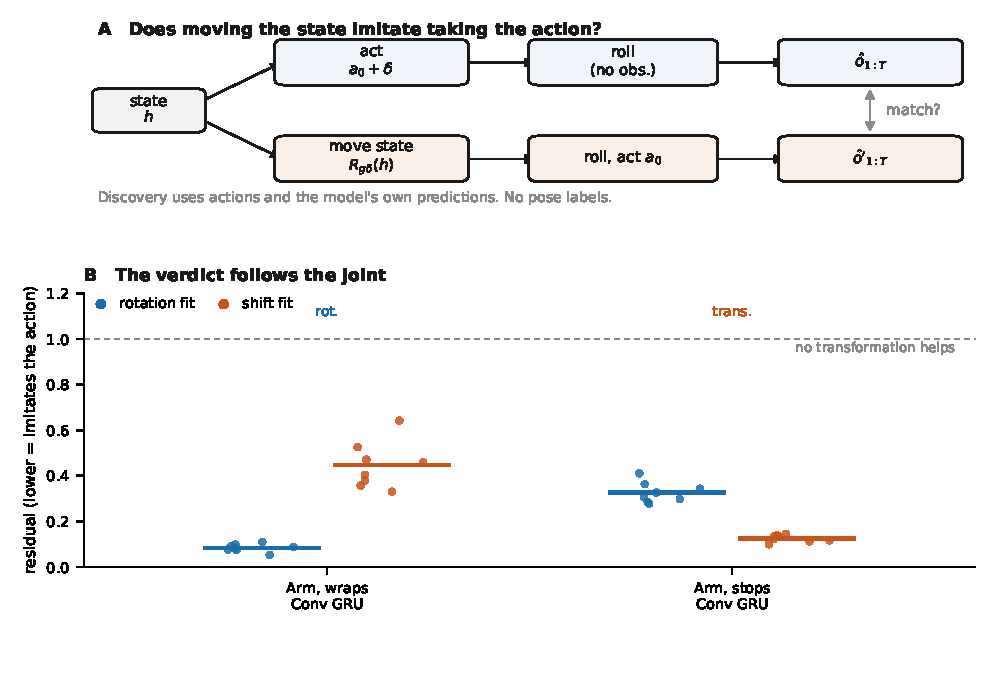
\includegraphics[width=\textwidth]{criterion.pdf}
\caption{
\textbf{A}: Action-conditioned test. From one latent state we compare a rollout after perturbing the action with a rollout after transforming the state, with observations withheld so both depend on the transition dynamics. A family matches the action when it reproduces the perturbed-action rollout.
\textbf{B}: The recovered transformation follows joint geometry. Wrapping joints give rotations, otherwise identical joints with stops give translations. \FIGCAPSPAN{} A residual near $1$ means the fitted transformation improves little on leaving the state unchanged.
}
\label{fig:criterion}
\end{figure}

Let $h_t$ denote the model's latent state, $a_t$ an action, and $\hat{o}$ a predicted observation. We withhold observations over a rollout window so that subsequent states depend only on the learned transition dynamics.

From the same state $h$ we generate two rollouts: the first perturbs the initial action by $\delta$, the second keeps the action fixed and transforms the initial latent state with $R$. We ask whether a single gain $g$ lets a transformation in the candidate family reproduce the perturbed-action rollout:

$$
\hat{o}_{1:T}\!\left(h,\,a_0+\delta\right)
\;\approx\;
\hat{o}_{1:T}\!\left(R_{g\delta}(h),\,a_0\right).
$$

The residual is the best prediction error achieved by the transformation divided by the error without transforming the state. A residual near $1$ means the candidate does not reproduce the action perturbation. Lower values indicate a stronger correspondence.

Discovery uses actions and the model's own predictions, not ground-truth joint labels. After discovery, we use the physical joint angles only to identify the recovered coordinate.

\paragraph{Transformation families.}
We test two one-parameter families matching common joint geometries. A freely wrapping joint has circular state, so its action is a rotation in a latent plane. A joint with stops lies on an interval, so its action is a translation along a direction. They differ before fitting: a translation gives a nonzero signed mean response, a rotation averages to zero across phase. We fit both and keep the lower residual.

\paragraph{Matched null.}
Low residuals can arise from flexible latent directions unrelated to the action. We therefore compare every fitted coordinate against directions from the orthogonal complement, matched for dimension and explained variance, asking whether it reproduces the action better than equally expressive directions.

\section{Results}

\subsection{Readable variables need not organize the dynamics}
\label{sec:dissoc}

In the serial two-joint arm of Section~\ref{sec:built}, both joints are visible and readable from the learned state: concentration $\SerialGruPOneKappa$ proximal and $\SerialGruPTwoKappa$ distal, against untrained floors of $\UntrGruPOneKappa$ and $\UntrGruPTwoKappa$, so the distal joint reads at roughly four times its floor.

The action-conditioned test gives a different result. The proximal joint reaches residual $\SerialGruPOneResid$ against a matched null of $\SerialGruPOneNull$, beating that null in $\SerialGruPOneBeats$ of $\nSerialSeeds$ seeds and falling below the lowest matched direction in $\SerialGruPOneStrict$. The distal joint reaches $\SerialGruPTwoResid$ against $\SerialGruPTwoNull$, with only $\SerialGruPTwoStrict$ seeds below that minimum. Mean margins are $\SerialGruPOneGap$ and $\SerialGruPTwoGap$.

Because the null is sampled, we repeated the analysis with an independent draw. The residuals are bit-identical, while the null medians move by $\SerialGruPOneNullDrift$ and $\SerialGruPTwoNullDrift$. The proximal margin stays $\SerialGruPOneMarginOverDrift$ times that variation and clears the null in $\SerialGruPOneBeatsA$ of $\nNullSeeds$ seeds under both draws. The distal count changes from $\SerialGruPTwoBeatsA$ to $\SerialGruPTwoBeatsB$ between draws. \HORIZONPARA

Only the proximal coordinate is clearly separated from null variability. We do not claim the distal plane carries nothing: at this sample size its residual is inconclusive, not negative. What differs is the strength of the two statements. Probe concentrations separate the joints by a factor of two and report both as readable. The action-conditioned margins separate them by a factor of six and establish only the proximal coordinate. Readability therefore does not settle whether the dynamics use a coordinate.

\subsection{Observation geometry determines the learned coordinates}
\label{sec:built}

\begin{table}[t]
\centering
\small
\caption{
Action space, joint dynamics, image size, sensor noise, architecture and training budget are held fixed while the observation's dependence on the two actuators changes. The criterion reports a residual with its matched-variance null in parentheses, and \emph{beats} counts seeds falling below their own null. The basis is discovered without angle labels, and concentration is measured afterwards against the named physical coordinate. $n=\nSerialSeeds$ seeds.
}
\label{tab:envs}
\begin{tabular}{llcccc}
\toprule
Environment & Image depends on & Basis & Residual (null) & Beats & Conc. \\
\midrule
Serial arm
& $q_1$ and $q_1{+}q_2$
& $\SerialGruPOneBasis$
& $\SerialGruPOneResid$ ($\SerialGruPOneNull$)
& $\SerialGruPOneBeats$/$\nSerialSeeds$
& $\SerialGruPOneKappa$ \\
Parity arm
& $q_1{+}q_2$ only
& $\ParityGruPOneBasis$
& $\ParityGruPOneResid$ ($\ParityGruPOneNull$)
& $\ParityGruPOneBeats$/$\nParitySeeds$
& $\ParityGruPOneKappa$ \\
Decoupled
& $q_1$ and $q_2$ separately
& $\DecoupGruPOneBasis$
& $\DecoupGruPOneResid$ ($\DecoupGruPOneNull$)
& $\DecoupGruPOneBeats$/$\nDecoupSeeds$
& $\DecoupGruPOneKappa$ \\
&
&
$\DecoupGruPTwoBasis$
& $\DecoupGruPTwoResid$ ($\DecoupGruPTwoNull$)
& $\DecoupGruPTwoBeats$/$\nDecoupSeeds$
& $\DecoupGruPTwoKappa$ \\
\bottomrule
\end{tabular}
\end{table}

A two-actuator system provides two independent action dimensions, but a predictive model need not give each actuator its own coordinate. We change only how the observation depends on the two actuators (Table~\ref{tab:envs}).

In the serial arm the image depends on the proximal angle $q_1$ and the absolute distal angle $q_1+q_2$, so proximal motion changes both links. The model learns one dominant coordinate aligned with the proximal joint, at residual $\SerialGruPOneResid$ against a null of $\SerialGruPOneNull$ in $\SerialGruPOneBeats$ of $\nSerialSeeds$ seeds. A second plane stays near its null, at $\SerialGruPTwoResid$ against $\SerialGruPTwoNull$.

A serial chain limits how strongly the distal actuator affects the image relative to the proximal one. Changing the link lengths moves the two toward parity, with the image-change ratio approaching $\envParityRatioOne$, at which point the image depends only on $q_1+q_2$. The model then learns a coordinate for that sum in $\ParityGruPOneVotes$ of $\nParitySeeds$ seeds, at concentration $\ParityGruPOneKSum$ against $\ParityGruPOneKProx$ for $q_1$ and $\ParityGruPOneKDist$ for $q_2$.

Giving each actuator a separate visible component, the model learns two coordinates, at residuals $\DecoupGruPOneResid$ and $\DecoupGruPTwoResid$ against nulls of $\DecoupGruPOneNull$ and $\DecoupGruPTwoNull$, beating their own nulls in $\DecoupGruPOneBeats$ and $\DecoupGruPTwoBeats$ of $\nDecoupSeeds$ seeds.

The action space is identical in all three environments, and the learned coordinate system changes with the variables the observation distinguishes. Predictive training organizes latent dynamics around observation geometry instead of assigning one coordinate per action dimension.

\subsection{The recovered transformation follows the physical state geometry}

The criterion should recover different families when the coordinate has different geometry, so we change whether the joints wrap and leave the rest of the environment unchanged. When the joints wrap it selects a rotation in $\FamParityGruPOneFamilyN$ of $\nFamParityGruSeeds$ seeds (residual $\FamParityGruPOneRot$ against $\FamParityGruPOneTra$ for a translation). Adding stops changes the coordinate from a circle to an interval, and the criterion then selects a translation in $\FamBoundGruPOneFamilyN$ of $\nFamBoundGruSeeds$ (residual $\FamBoundGruPOneTra$ against $\FamBoundGruPOneRot$; Figure~\ref{fig:criterion}B).

\ARCHPARA

\DOMAINPARA

\VALIDITYPARA

\section{Limitations}

\LIMSCOPE{}

Our models have fewer than four million parameters and our environments are simulated, so the experiments establish a controlled separation between readability and dynamic use without estimating how often it appears in deployed systems. The criterion tests two one-parameter families and will not detect coordinates governed by other transformations.

Readability is measured against an untrained-network floor, not a tuned probe, so a comparison with stronger probing and disentanglement methods \citep{higgins2017betavae,locatello2019challenging} remains open. The experiments establish that high concentration can coexist with weak action-conditioned evidence, not that the criterion dominates every alternative measure. Inference is across seeds at an exact two-sided sign-flip floor of $p=\exactFloor$, which is why we report effect sizes and matched-null margins alongside it.

\section{Conclusion}

A readable variable and a dynamically active coordinate are different properties of a world model. We test the second by asking whether a transformation of the latent state reproduces the model's response to an action perturbation. In controlled two-joint environments the criterion separates coordinates that probes call similarly present, and observation geometry determines which coordinates predictive training builds. For robot learning this is a concrete constraint: predictive objectives organize latent dynamics around distinctions available in the observation, so a task needing separate control-relevant coordinates must have an observation or objective that distinguishes them.

\bibliographystyle{plainnat}
\bibliography{refs}

\end{document}
